\documentclass[conference]{IEEEtran}
\usepackage{graphicx}
	\setkeys{Gin}{width=0.4\textwidth}
\usepackage{enumitem}
\hyphenation{op-tical net-works semi-conduc-tor}


\begin{document}
\title{Feature selection in heart disease diagnosis}

% author names and affiliations
% use a multiple column layout for up to three different
% affiliations
\author{\IEEEauthorblockN{Juan Aceron, Marc Teves, Thomas Saliba}
\IEEEauthorblockA{Department of Computer Science\\College of Engineering\\University of the Philippines, Diliman}}

\maketitle

\begin{abstract}
	Assessing the severity of heart disease in a patient is important.
	Machine learning algorithms can solve this problem by considering risk factors and their correlation with the presence of heart disease.
	Most machine learning algorithms suffer the curse of dimensionality, wherein the time taken to fit a model with training data suffers as the number of features increases.
	In addition, having more features tends to overfit the model with the data.
	To avoid the problems with excessive features, feature selection, also known as feature ranking, is employed to reduce features in datasets with large amounts of features.
	The group uses the naive approach of feature selection, evaluating the performance of each element in the powerset of the feature set.
	Performance is taken as the weighted average of each non-diagonal cell in a confusion matrix, so that more severe false negative cases have a higher weight.
	In the case of assessing heart disease, each feature is extracted using medical procedures with varying cost.
	This is taken into account when selecting the best feature set, so as to obtain the feature set that is most effective computationally, and in terms of cost.
	The group found that (feature set) is the most effective in terms of performance, saving up to (result) in medical costs per diagnosis.
\end{abstract}

\section{Introduction}
	Heart disease, particularly coronary heart disease (CHD), is the leading cause of death among adults in the industrialized world \cite{bib:stroke_stat}.
	CHD and stroke are life threatening conditions which require expensive treatments when they occur.
	When diagnosed correctly and prevented, the preventative measures for CHD and stroke do not cost much.
	If heart disease is prevented from progressing, there will be a lot of money saved in medical treatments.

	Zethraeus et. al.\cite{bib:stroke_save} estimated that in 1999 in Sweden, preventing the onset of CHD or stroke saved each patient a medical bill ranging from 36 000 SEK to 91 000 SEK.
	In today's money, that would range from 274348 Php to 693498 Php per stroke prevented. \cite{bib:secpi}

	Preventing and accurately diagnosing heart disease risk factors translates to major savings in medical fees.
	Getting checked for heart disease is the same as almost any other medical diagnosis.
	The patient is subjected to various non-invasive medical tests with varying prices.
	For example, finding the patient's cholesterol levels will cost 7.27 CAD, while finding the maximum heart rate achieved through a thalium stress test costs 102.90 CAD. \cite{bib:dataset}

	After receiving the tests, a trained medical professional decides whether or not the patient has heart disease, and the severity of said heart disease.

	Machine learning approaches have been proposed to automate the task of diagnosing heart disease.\cite{bib:dataset} \cite{bib:mltech}
	Ultimately, this is a data analysis problem.
	A common theme with data analysis is the \emph{curse of dimensionality}.
	As the number of features grows in a dataset, the predictive power of the model used to characterize it increases up until a point where it starts to decrease. \cite{bib:curse}
	With the case of machine learning, the time taken to fit the model with the data increases, for diminishing returns in performance.
	It would be helpful if only the most relevant and most predictive features are selected for data analysis.

	This problem can be solved with \emph{feature selection}, or \emph{feature ranking}.
	Feature selection is the task of selecting the best subset of features from a given dataset that will create the best predictor, in terms of performance.

	Medical diagnosis problems will benefit not only in training time and accuracy of their predictive models, but in saving diagnosis cost as well, since the number of tests will be reduced for each patient.

	In this project, the best performing subset of features will be selected using naive feature selection.
	The subset of features will be evaluated by their performance in a support vector machine (SVM).
	
	In addition, the best feature sets will be evaluated at price intervals.

\section{Short of Review of Related Studies}
	The Cleveland heart disease dataset is a well-known dataset used for the heart disease diagnosis problem.
	Many SVM models have been created to analyze this dataset.

	Khanna et. al. \cite{bib:mltech} created an SVM model with an F-score of 0.87.
	However they did not provide a detailed methodology.
	They also did not do any feature selection.

	Nahar et. al. \cite{bib:smo} used two techniques of feature selection: 
	manual (MFS) and computerized (CFS).

	Without feature selection, their SMO classifier got an F-score of 0.862.
	With MFS, it got an F-score of 0.8.
	With CFS, it got an F-score of 0.815.
	Taking the intersection of feature subsets (MFS+CFS), the SMO classifier got an F-score of 0.861.

	Compared to the full feature set, the SMO model seemed to do worse after MFS+CFS.
	The loss in performance is insignificant compared to the savings in medical fees by taking the reduced 3-feature subset as a basis for predictive models, instead of the 14-feature feature set.
	Nahar concluded that chest pain type, maximum heart rate, and exercise induced angina are the best features to use to decrease training time and decreasing medical cost.
	This study points to the idea that reducing the feature set will not incurr significant losses in performance.

\section{Methodology and Results}
	The dataset used for the SVM classifier was the Cleveland heart disease dataset.
	The dataset has 76 features but only 14 are ever used. These are:
	\begin{enumerate}[start=0]
	  \item age - in years
      \item sex - sex of subject     
      \item cp - chest pain type
      \item trestbps - resting blood pressure
      \item chol - serum cholesterol in mg/dl
	  \item fbs - boolean measure indicating whether fasting blood sugar is greater than 120 mg/dl
      \item restecg - resting ECG type
      \item thalach - maximum heart rained attained
      \item exang - boolean measure indicating whether or not exercise induced angina
      \item oldpeak - ST depression brought by exercise relative to rest
      \item slope - the slope of the ST segment for peak exercise
	  \item ca - number of major vessels (0 - 3) colored by fluoroscopy        
      \item thal - the heart status (normal, fixed defect, reversible defect) (nominal) 
	  \item num - the class attribute (0 - 4) 
	\end{enumerate}
	A processed copy of the dataset is included in the website it was retrieved from, with only the relevant features included and all data converted into numerical forms.
	Because of this, there was no need for preprocessing.

	Overall, there are 13 features used to predict the last column, the class attribute.
	A powerset of the feature set is obtained, and each element in that powerset (except for the zero features) is used to train an SVM.
	The performance of the SVM is measured using F-score, so that precision andrecall are given equal importance.

	The classifiers used the RBF kernel type.
	RBF was chosen because previous trials with the polynomial kernel had a poorer performance than the RBF kernel type, and according to Tien Lin \cite{bib:rbf} RBF is a good general purpose kernel type.

	For the most cost effective set of features, one is selected for each price range.

	Looking at Figure~\ref{fig:cost_graph}, the most sensible price ranges chosen for the experiment are: (0, 50], (50, 150], (150, 250], (250, 350], (350, 450], (450, 550], (550, 650].
	Each feature set belongs to one price range. One feature set with the highest performing SVM classifier will be selected for each price range.
	In case of a tie in F-score, the cheaper feature set is chosen.

	\begin{figure}[h]
		\centering
		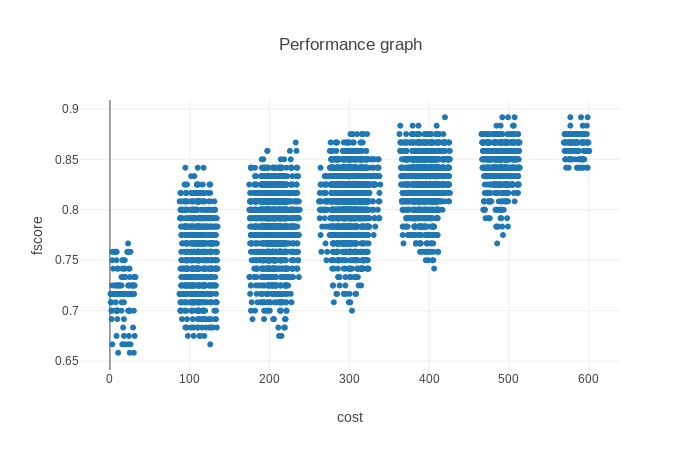
\includegraphics{cost_vs_fscore.png}
		\caption{Cost vs. F-score graph. Notice the clustering around multiples of 100}
		\label{fig:cost_graph}
	\end{figure}

	Given Figure~\ref{fig:feat_graph}, we expect to find the best performing
	feature sets to have a length of 7, 8, or 9.

	\begin{figure}[h]
		\centering
		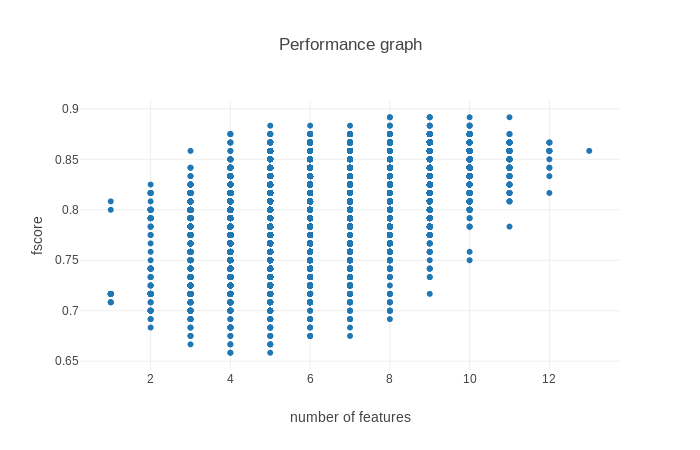
\includegraphics{features_vs_fscore.png}
		\caption{Feature number vs. F-score graph.}
		\label{fig:feat_graph}
	\end{figure}

	The most cost effective SVM classifiers for each price range are given in
	Figure~\ref{fig:cost_effective}. Looking at the table, we see that the 
	best feature set in terms of F-score are tied at the three highest 
	price ranges. As the cheapest high performance feature set, it seems that
	the feature set \texttt{(1, 2, 3, 4, 6, 7, 9, 11, 12)} is the best.
	This feature set has 9 features.

	By removing the need for testing \texttt{slope} and replacing it with \texttt{fbs}, up to 72 CAD was saved between the best candidate in (350, 450] and (450, 550].

	Even bigger savings were earned between (350, 450] and (550, 650].

	\begin{figure*}[h]
		\begin{tabular}[h]{|c|c|c|c|}
			\hline
			Price Range & Feature Set & Cost & F-score \\ \hline
			(0, 50] & (0, 2, 5, 6) & 22.7 & 0.767 \\ \hline
			(50, 150] & (1, 2, 5, 10) & 94.5 & 0.842 \\ \hline
			(150, 250] & (2, 4, 5, 6, 11, 12) & 232.77 & 0.867 \\ \hline
			(250, 350] & (1, 2, 3, 4, 7, 10, 11) & 301.37 & 0.875\\ \hline
			(350, 450] & (1, 2, 3, 4, 6, 7, 9, 11, 12) & 419.77 & 0.892 \\ \hline
			(450, 550] & (1, 2, 3, 4, 7, 8, 9, 11, 12) & 491.57 & 0.892 \\ \hline
			(550, 650] & (2, 4, 7, 8, 9, 10, 11, 12) & 576.87 & 0.892 \\ \hline
			\hline
		\end{tabular}
		\centering
		\label{fig:cost_effective}
		\caption{Table of best feature sets belonging to each price interval}
	\end{figure*}

	\begin{figure}[h]
		\centering
		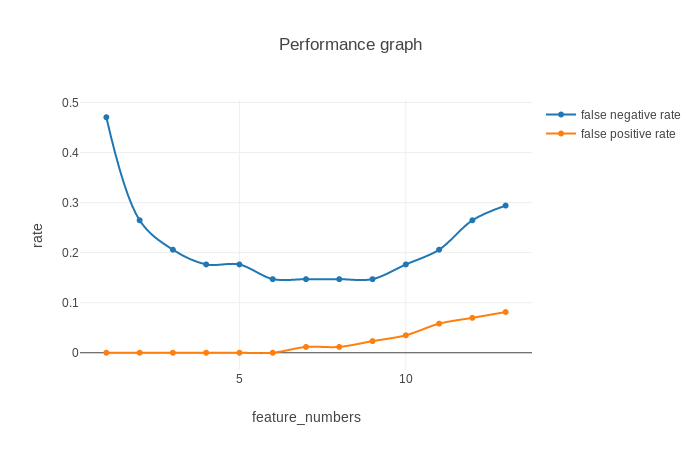
\includegraphics{fn_fp_rate.png}
		\caption{Error rate graph.}
		\label{fig:fn_rate}
	\end{figure}

	Starting from the lowest number of features, the false negative rate starts at 100\%, decreasing as the number of features increases.
	This can be seen in Figure~\ref{fig:fn_rate}.
	This graph shows a plot (in blue) of the lowest false negative rates found for each group of feature sets with the length found at the x-axis.

	In the same figure, another plot (in orange) shows the lowest false positive rates found for each group of feature sets with the length found at the x-axis.
	This plot stays at zero up until $x=6$, where it begins rising.

	These two plots paint the same picture: all of the SVM models are biased
	towards selecting negatives rather than a positive.
	That is, the models generated from our approach are prone to false negatives.
	This is especially harmful in medical diagnosis, where the more favorable tradeoff is lowering false negatives if it means increasing false positives.
	The lowest false negative rate was found at $x=6,7,8$, however it is notable that the overall best feature set chosen had a feature length of 9.

	This bias towards a negative decision might be caused by the dataset being imbalanced in favor of negative instances.

\section{Conclusion}
	The group was able to create an SVM classifier for the heart disease diagnosis problem with an F-score of 0.892.
	It was proven that reducing the feature set can increase the performance of a classifier.

	Moreover, the group proved that a more expensive procedure does not equate to a better diagnosis.
	By removing certain features and substituting them in favor of features obtained with less expensive procedures, an accuracy similar to the expensive procedure can be achieved.

	A recommendation for future studies is to deal with the problems caused by an imbalanced dataset.

\begin{thebibliography}{1}

\bibitem{bib:stroke_stat}
	American Heart Association. \emph{Heart Disease and Stroke Statistics—2003
		Update}. Dallas, Tex: American Heart Association; 2002.
\bibitem{bib:stroke_save}
	Zethraeus N, Molin T, Henriksson P, Jönsson B. \emph{Costs of coronary heart disease and stroke: the case of Sweden}. J Intern Med. 1999;246(2):151-9.
\bibitem{bib:secpi}
	Swedish Consumer Board. \emph{CPI, Fixed Index Numbers (1980=100)}. Statistics Sweden. 2018
\bibitem{bib:dataset}
Detrano,~R., Janosi,~A., Steinbrunn,~W., Pfisterer,~M., Schmid,~J.,
       Sandhu,~S., Guppy,~K., Lee,~S., \& Froelicher,~V. (1989).  {\it 
       International application of a new probability algorithm for the 
       diagnosis of coronary artery disease.}  {\it American Journal of 
       Cardiology}, {\it 64},304--310.
\bibitem{bib:mltech}
	D. Khanna, R. Sahu, V. Baths, and B. Deshpande. \emph{Comparative Study of Classification Techniques (SVM, Logistic Regression and Neural Networks) to Predict the Prevalence of Heart Disease}. International Journal of Machine Learning and Computing, vol.5, no. 5, pp. 414-419, 2015.
\bibitem{bib:curse}
	Trunk, G. V. (July 1979). \emph{A Problem of Dimensionality: A Simple Example}. IEEE Transactions on Pattern Analysis and Machine Intelligence. PAMI-1 (3): 306–307.
\bibitem{bib:smo}
	Nahar, J., Imam, T., Tickle, K. S., \& Chen, Y.-P. P. (2013). \emph{Computational intelligence for heart disease diagnosis: A medical knowledge driven approach}. Expert Systems with Applications, 40(1), 96–104. https://doi.org/10.1016/j.eswa.2012.07.032 
\bibitem{bib:rbf}
	Tien Lin H., Jen Lin C., \emph{A Study on Sigmoid Kernels for SVM and the Training of non-PSD Kernels by SMO-type Methods}. Department of Computer Science and Information Engineering. National Taiwan University

\end{thebibliography}




% that's all folks
\end{document}


